%!TEX platex=1
\documentclass[11pt,xcolor=dvipsnames,table,dvipdfmx,aspectratio=169]{beamer}
\usepackage{amsmath, amssymb}
\usepackage{latexsym}
\usepackage{ascmac}
\usepackage{bm}

%$B%-%c%W%7%g%s@_Dj(B
\usepackage{caption}
\captionsetup[figure]{font=scriptsize}

%Beamer$B$N@_Dj(B
\usetheme{Boadilla}
%Beamer$B%U%)%s%H@_Dj(B
\usepackage{txfonts} % TX$B%U%)%s%H(B
\usepackage[deluxe]{otf} % $BF|K\8lB?%&%'%$%H2=(B
\renewcommand{\familydefault}{\sfdefault}  % $B1QJ8$r%5%s%;%j%UBN$K(B
\renewcommand{\kanjifamilydefault}{\gtdefault}  % $BF|K\8l$r%4%7%C%/BN$K(B
\usefonttheme{professionalfonts}
\setbeamerfont{alerted text}{series=\bfseries} % Alert$B$rB@;z(B
\setbeamerfont{section in toc}{series=\mdseries} % $BL\<!$OB@;z$K$7$J$$(B
\setbeamerfont{frametitle}{size=\Large} % $B%U%l!<%`%?%$%H%kJ8;z%5%$%:(B
\setbeamerfont{title}{size=\LARGE} % $B%?%$%H%kJ8;z%5%$%:(B
\setbeamerfont{date}{size=\small}  % $BF|IUJ8;z%5%$%:(B

%Beamer$B?'@_Dj(B
\definecolor{UniBlue}{RGB}{0,150,200} 
\definecolor{AlertOrange}{RGB}{255,76,0}
\definecolor{AlmostBlack}{RGB}{38,38,38}
\setbeamercolor{normal text}{fg=AlmostBlack}  % $BK\J8%+%i!<(B
\setbeamercolor{structure}{fg=UniBlue} % $B8+=P$7%+%i!<(B
\setbeamercolor{block title}{fg=UniBlue!50!black} % $B%V%m%C%/ItJ,%?%$%H%k%+%i!<(B
\setbeamercolor{alerted text}{fg=AlertOrange} % \alert $BJ8;z%+%i!<(B
\mode<beamer>{
    \definecolor{BackGroundGray}{RGB}{254,254,254}
    \setbeamercolor{background canvas}{bg=BackGroundGray} % $B%9%i%$%I%b!<%I$N$_GX7J$r$o$:$+$K%0%l!<$K$9$k(B
}

% $BCm<a$r(B 1) 2) 3)$B$N7A<0$KJQ99(B
\renewcommand\thefootnote{\arabic{footnote})}

% Algorithm$B7O(B
\usepackage{algorithm}
\usepackage[noend]{algpseudocode}
\renewcommand\algorithmicrequire{\textbf{Input:}}
\renewcommand\algorithmicensure{\textbf{Output:}}

%$B%^%/%m(B
\def\rank{\mathop{\rm rank}}
\def\Re{\mathop{\rm Re}}
\def\Im{\mathop{\rm Im}}
\def\N{\mathbb{N}}
\def\diag{\mathop{\rm diag}}
\def\blockdiag{\mathop{\rm block\ diag}}
\def\bedr{\hfill $\Box$}
\def\trace{\mathop{\rm tr}}
\def\R{\mathbb{R}}
\def\P{\mathop{\rm P}}
\def\C{\mathbb{C}}
\def\I{\mathcal{I}}
\def\B{\mathcal{B}}
\def\D{\mathcal{D}}
\def\T{\mathop{\rm T}}
\def\H{\mathop{\rm H}}
\def\elig{{\rm Elig}}
\def\wx{\widetilde x}
\def\tx{\tilde x}
\def\Vec#1{\mbox{\boldmath $#1$}}
\def\v#1{\mbox{\boldmath $#1$}}
\def\defspace{$\vspace*{0.5mm}$}
\def\E{\mathop{\rm E}}
\def\Var{\mathop{\rm Var}}
\def\tr{\mathop{\rm tr}}
\def\sm{\setminus}
\def\hs{\hspace{0.2cm}}

%$B%U%i%C%H%G%6%$%s2=(B
\setbeamertemplate{blocks}[rounded] % Block$B$N1F$r>C$9(B
\useinnertheme{circles} % $B2U>r=q$-$r%7%s%W%k$K(B
\setbeamertemplate{navigation symbols}{} % $B%J%S%2!<%7%g%s%7%s%\%k$r>C$9(B
\setbeamertemplate{footline}[frame number] % $B%U%C%?!<$O%9%i%$%IHV9f$N$_(B

%$B%?%$%H%k%Z!<%8(B
\setbeamertemplate{title page}{%
    \vspace{2.5em}
    {\usebeamerfont{title} \usebeamercolor[fg]{title} \inserttitle \par}
    {\usebeamerfont{subtitle}\usebeamercolor[fg]{subtitle}\insertsubtitle \par}
    \vspace{1.5em}
    \begin{flushright}
        \usebeamerfont{author}\insertauthor\par
        \usebeamerfont{institute}\insertinstitute \par
        \vspace{3em}
        \usebeamerfont{date}\insertdate\par
        \usebeamercolor[fg]{titlegraphic}\inserttitlegraphic
    \end{flushright}
}

% graphicx.sty
\usepackage{graphicx}

%
\def\qed{\hfill $\Box$}

\AtBeginSection[]{
    \frame{\tableofcontents[currentsection, hideallsubsections]} %$BL\<!%9%i%$%I(B
}

%$B%?%$%H%k(B
\title{$k$$B:GC;O)$NC5:w(B}
\author{\textbf{$BK\EDM:0lO:(B}}
\date{2017/01/30}
\institute{$BBg:eBg3X>pJs2J3X8&5f2J(B\\$B>pJs?tM}3X@l96(B $B?9ED8&5f<<(B M1}

\usepackage{multicol}	% required for `\multicols' (yatex added)
\begin{document}
\maketitle

\begin{frame}{$B>R2p$9$kO@J8(B}
 D.Eppstein: ``Finding the {\it k} shortest paths'' SIAM Journal on Computing 28(2) (1997)
\end{frame}

\begin{frame}{$BLdBj@_Dj(B}
  \begin{block}{$BLdBj(B}
  \textbf{Input:}
  \begin{itemize}
   \item $G = (E, V)$: $BM-8~%0%i%U(B
   \item $c: E \rightarrow R_+$: $B@5$NJU=E$_4X?t(B
   \item $s, t \in V$: $B;OE@!$=*E@(B
  \end{itemize}
  \textbf{Output:}
  \begin{itemize}
   \item $p_1, p_2, ..., p_k$: $1$$B!A(B$k$$B:GC;O)(B
  \end{itemize}
 \end{block}
\end{frame}

\begin{frame}{$B<g7k2L(B}
 \begin{block}{$B<g7k2L(B}
  $B%0%i%U(B$G$$B$K$*$1$k(B$s$$B$+$i(B$t$$B$X$N(B$1$$B!A(B$k$$B:GC;O)$r(B$O(m + n\log n + k)$$B$GNs5s$G$-$k!%(B
 \end{block}
\end{frame}

\begin{frame}{$B<j=g(B}
 $BBg$^$+$K$O0J2<$NN.$l$G(B$k$$B:GC;O)$r5a$a$k$?$a$N%0%i%U(B$P(G)$$B$r:n@.$9$k!%(B
 \begin{enumerate}
  \item $B:GC;O)LZ(B$T$$B$N:n@.!%(B($O(m + n \log n)$)
  \item 2$B$D$N(B2$BJ,%R!<%W$NB2(B$H_{out}(v)$$B!$(B$H_T(v) \hs (v \in V)$$B$r:n@.!%(B($O(m)$$B!$(B$O(n \log n)$)
  \item $H_{out}(v)$$B!$(B$H_T(v)$$B$r%^!<%8$7$F(B3$BJ,%R!<%W$+$i$J$kHs=d2s%0%i%U(B$D(G)$$B$r:n@.!%(B($O(n \log n)$)
  \item $D(G)$$B$KJU$HD:E@$rDI2C$7!$(B4$BJ,%R!<%W$+$i$J$k%0%i%U(B$P(G)$$B$r:n@.!%(B($O(m + n \log n)$)
 \end{enumerate}
\end{frame}

\begin{frame}{$BMQ8l@0M}(B}
 \begin{itemize}
  \item $d(u, v)$:\hs $BD:E@(B$u$$B$+$iD:E@(B$v$$B$X$N:GC;O)$N5wN%(B
  \item $l(e)$:\hs $BJU(B$e$$B$ND9$5(B
  \item $tail(e)$$B!$(B$head(e)$:\hs $BM-8~JU(B$e$$B$N;OE@!$=*E@(B
  \item $\delta(e) := l(e) + d(head(e), t) - d(tail(e), t)$:\hs $e$$B$rDL$C$?$3$H$K$h$k:GC;O)$H$N:9(B
 \end{itemize}
\end{frame}

\begin{frame}{$BM-8~%0%i%U(B$G$$B$H:GC;O)LZ(B$T$}
 \begin{figure}[htbp]
  \begin{minipage}{0.3\hsize}
   \centering
   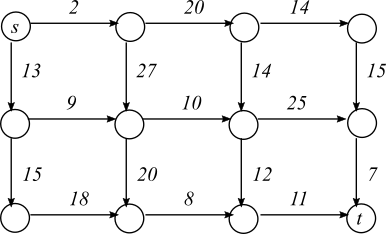
\includegraphics[width=5cm]{graphG.png}
   \caption{$G$}
  \end{minipage}
  \begin{minipage}{0.2\hsize}
   \centering
   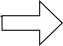
\includegraphics[width=0.75cm]{rightarrow.png}
  \end{minipage}
  \begin{minipage}{0.3\hsize}
   \centering
   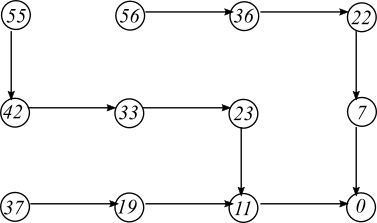
\includegraphics[width=5cm]{shortestPathTreeT.png}
   \caption{$B:GC;O)LZ(B$T$}
  \end{minipage}
 \end{figure}
 \begin{itemize}
  \item $G$$BFb$G!$(B$t$$B$+$i5U8~$-$K(BDijkstra$BK!$rE,MQ$9$k$3$H$G(B$T$$B$rF@$k!%(B($O(m + n \log n)$)
  \item $T$$B$N3FD:E@$N=E$_$O(B$t$$B$+$i$N5wN%!%(B
  \item $T$$BFb$GD:E@(B$v$$B$N<!$KMh$kD:E@$r(B$next_T(v)$$B$HI=$9!%(B
 \end{itemize}
\end{frame}

\begin{frame}{$G-T$$B$H(B$sidetracks$}
 \begin{figure}[htbp]
  \begin{minipage}{0.4\hsize}
   \centering
   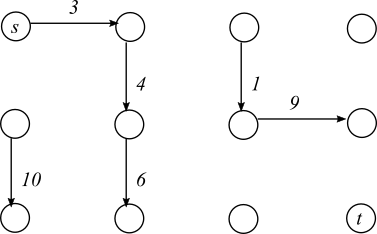
\includegraphics[width=5cm]{G-T.png}
   \caption{$G-T$}
  \end{minipage}
  \hspace{1cm}
  \begin{minipage}{0.4\hsize}
   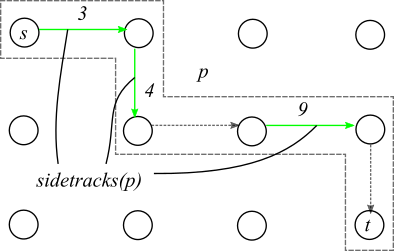
\includegraphics[width=5cm]{sidetracks.png}
   \caption{$sidetracks(p)$}
  \end{minipage}
 \end{figure}
 $G$$BFb$N(B$s-t$$BF;(B$p$$B$,M?$($i$l$?$H$-!$JU=89g(B$sidetracks(p)$$B$r<!$N$h$&$KDj$a$k!%(B
 \begin{align*}
   sidetracks(p) = \{e|\hs e \in G-T, e \in p\}
 \end{align*}
 $G-T$$BFb$N(B$sidetracks(p)$$B$O(B$G$$BFb$N(B$s-t$$BF;(B$p$$B$H(B1$BBP(B1$B$KBP1~$9$k!%(B
\end{frame}

\begin{frame}{2$B$D$N%R!<%W$N:n@.(B(1)}
 \begin{figure}[htbp]
  \begin{minipage}{0.3\hsize}
   \centering
   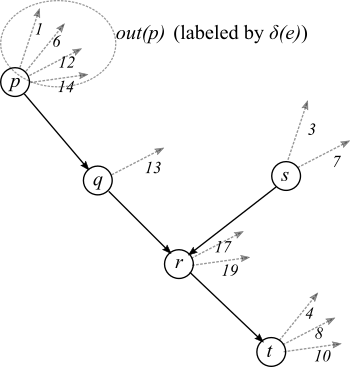
\includegraphics[width=5cm]{portionOfT.png}
   \caption{$B:GC;O)LZ(B$T$$B$NItJ,%0%i%U(B}
  \end{minipage}
  \begin{minipage}{0.2\hsize}
   \centering
   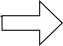
\includegraphics[width=0.75cm]{rightarrow.png}
  \end{minipage}
  \begin{minipage}{0.3\hsize}
   \centering
   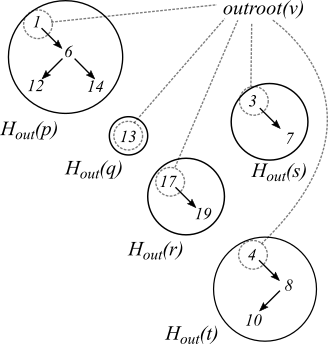
\includegraphics[width=5cm]{Hout(v).png}
   \caption{$H_{out}(v)$}
  \end{minipage}
 \end{figure}
 \begin{itemize}
  \item $B3FD:E@(B$v$$B$K$D$$$F!$(B$(v, w) \in G-T$$B$H$J$k:G>.$NJU(B($B0J8e!$(B$outroot(v)$$B$H8F$V(B)$B$r<h$j=P$7!$;D$j$NJU$G%R!<%W$r:n$k!%:n@.$7$?%R!<%W$N:,$r(B$outroot(v)$$B$N1&$N;R$H$9$k!%(B($O(m)$)
 \end{itemize}
\end{frame}

\begin{frame}{2$B$D$N%R!<%W$N:n@.(B(2)}
 \begin{figure}[htbp]
  \begin{minipage}{0.3\hsize}
   \centering
   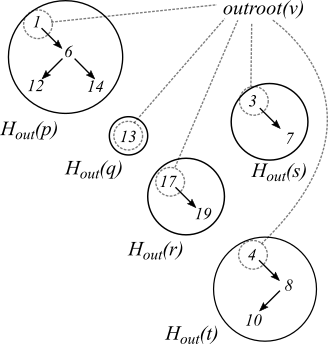
\includegraphics[width=5cm]{Hout(v).png}
   \caption{$H_{out}(v)$}
  \end{minipage}
  \begin{minipage}{0.2\hsize}
   \centering
   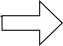
\includegraphics[width=0.75cm]{rightarrow.png}
  \end{minipage}
  \begin{minipage}{0.3\hsize}
   \centering
   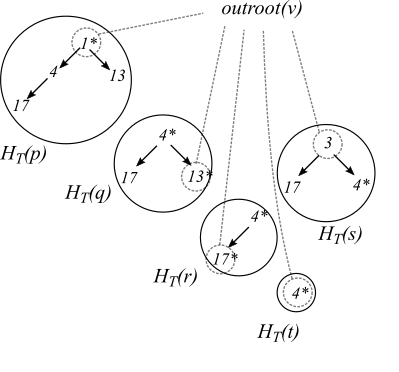
\includegraphics[width=5.5cm]{HT(v).png}
   \caption{$H_T(v)$}
  \end{minipage}
 \end{figure}
 \begin{itemize}
  \item $H_T(t) := {outroot(t)}$$B!%(B$H_T(next_T(v))$$B$K(B$outroot(v)$$B$rA^F~$7(B$H_T(v)$$B$r9=@.!%(B($O(n\log n)$)
  \item $H_{out}(v)$$B!$(B$H_T(v)$$B$ND:E@$O%0%i%U(B$G$$B$NJU$H(B1$BBP(B1$B$KBP1~$9$k$3$H$KCm0U!%(B
 \end{itemize}
\end{frame}

\begin{frame}{$D(G)$$B$+$i(B$P(G)$$B$N9=@.$X(B}
  \begin{figure}[htbp]
  \begin{minipage}{0.3\hsize}
   \centering
   \vspace{0.7cm}
   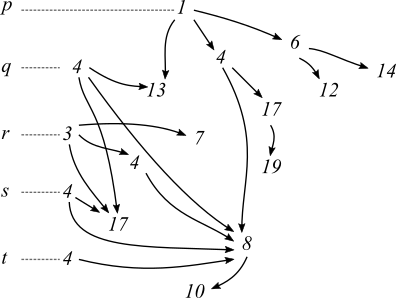
\includegraphics[width=5cm]{D(G).png}
   \caption{$BM-8~Hs=d2s%0%i%U(B$D(G)$}
  \end{minipage}
  \begin{minipage}{0.2\hsize}
   \centering
   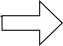
\includegraphics[width=0.75cm]{rightarrow.png}
  \end{minipage}
  \begin{minipage}{0.3\hsize}
   \centering
   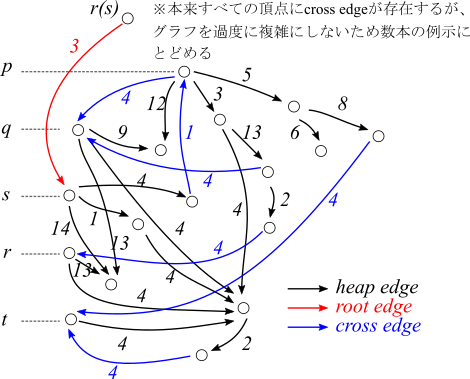
\includegraphics[width=6cm]{P(G).png}
   \caption{$B%0%i%U(B$P(G)$}
  \end{minipage}
 \end{figure}
 \begin{itemize}
  \scriptsize
  \item $B%R!<%W(B$H_T(v)$$B!$(B$H_{out}(v)$$B$r%^!<%8$7$F%0%i%U(B$D(G)$$B$r:n@.!%!J(B$D(G)$$B$ND:E@$N=P<!?t$O9b!9(B3$B$H$J$k$3$H$KCm0U!K(B
  \item $D(G)$$B$K:,$H$J$kD:E@(B$r(s)$$B$rDI2C$7!$(B$r(s)$$B$+$i(B$h(s):=outroot(s)$$B$X$NJU=E$_$r(B$\delta(h(s))$$B$H$9$k!%(B
  \item $D(G)$$BFb$NJU(B$(u, v)$$B$N=E$_$r(B$\delta(v)-\delta(u)$$B$GDj$a$k!%(B
  \item $D(G)$$BFb$ND:E@(B$p$$B$,BP1~$9$k(B$G$$BFb$NJU(B$(x, y)$$B$KBP$7!$JU(B$(p, h(y))$$B$r(B$D(G)$$BFb$KDI2C$7!$=E$_$r(B$\delta(h(y))$$B$GDj$a$k!%(B
  \item $P(G)$$B$O1&?^$NMM$K$J$k(B($B"((B)$B!%$J$*!$>e5-$N:n6H$OA4$F(B$O(m + n \log n)$$B$G9T$($k$3$H$KCm0U!%(B
 \end{itemize}
\end{frame}

\begin{frame}{$P(G)$$B$N@-<A(B}
 \begin{enumerate}
  \item $P(G)$$B$O(B$O(m + n \log n)$$B8D$ND:E@$r;}$D!%(B
  \item $P(G)$$B$ND:E@$N=P<!?t$O9b!9(B$4$$B$G$"$k!%(B
  \item $P(G)$$B$NJU$OHsIi$N=E$_$r;}$D!%(B
  \item $G$$BFb$N(B$s-t$$BF;$H(B$P(G)$$BFb$N(B$r$$B$+$i=PH/$7$?F;$O(B1$BBP(B1$B$KBP1~$9$k!%(B
  \item $P(G)$$BFb$NF;(B$p'$$B$N=E$_$r(B$l$$B$H$9$k$H!$BP1~$9$k(B$G$$BFb(B$s-t$$BF;(B$p$$B$N=E$_$O(B$d(s, t)+l$$B$GI=$;$k!%(B
 \end{enumerate}
\end{frame}

\begin{frame}{$B%R!<%W$K4X$9$kJdBj(B}
 \begin{block}{$BJdBj(B (Frederickson, 1993)}
  2$BJ,%R!<%WFb$N(B$k$$BHVL\$K>.$5$$MWAG$r(B$O(k)$$B$G<hF@$G$-$k!%(B
 \end{block}
 \begin{exampleblock}{4$BJ,%R!<%W$+$i(B2$BJ,%R!<%W$X$NJQ7A(B}
  \begin{figure}
   \centering
   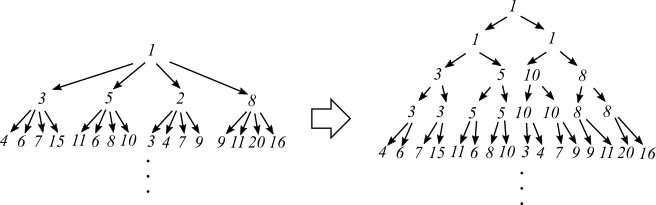
\includegraphics[width=14cm]{4heap2binaryheap.png}
  \end{figure}
 \end{exampleblock}
\end{frame}

\begin{frame}{Reference}
 \begin{thebibliography}{9}
  \bibitem{1} D.Eppstein: ``Finding the {\it k} shortest paths'' SIAM Journal on Computing 28(2) (1997)
  \bibitem{2} G.N.Frederickkson: ``An optimal algorithm for selection in a min-heap'' Information and Computation 104 (1993)
 \end{thebibliography}
\end{frame}

\begin{frame}{Appendix}
 \begin{block}{$P(G)$$B$N@-<A$N>ZL@(B}
  \scriptsize
  1: $v \in V$$B$KBP$7!$(B(i)$H_T(v)$$B$ND:E@$N$&$A%i%Y%k$,IUM?$5$l$?$b$N$H!$(B(ii)$H_{out}(v)$$BFb$ND:E@A4$F$H!$(B(iii)$r(s)$$B$,(B$P(G)$$B$ND:E@$H$J$k!%(B\\ \hs\hs(i)$B$O(B$O(\sum_{k=1}^{n}\log k) = O(n\log n)$$B!$(B(ii)$B$O(B$O(m)$$B!$(B(iii)$B$O(B$O(1)$$B$G$"$k$+$i!$(B$O(V(P(G))) = O(m + n \log n)$$B!%(B\\
  2: $D(G)$$B$N=P<!?t$,9b!9(B3$B$G$"$k$3$H$H!$3FD:E@$,(B1$BK\$@$1(B$cross edge$$B$r;}$D$3$H$+$iL@$i$+!%(B\\
  3: $D(G)$$B$,%R!<%W$G$"$k$N$G!$3FJU(B$(u, v)$$B$O(B$\delta(v)-\delta(u)\geq 0$$B$rK~$?$9!%$^$?!$(B$G$$B$NJU=E$_$,HsIi$G$"$k$N$G(B$\forall v \in P(G);\, \delta(h(v))\geq 0$$B!%(B\\
  4$B!$(B5: $B>JN,(B
 \end{block}
\end{frame}

\end{document}